\documentclass[11pt,a4paper,english]{article}
\usepackage[T1]{fontenc}
\usepackage[utf8]{inputenc}
\usepackage{babel}
\usepackage{geometry}
    \geometry{
    	left=2cm,
	right=2cm,
	includeheadfoot, top=1cm, bottom=1cm,
    headsep=2cm,
    footskip=2.5cm
    }
\usepackage{fancyhdr}
\usepackage{lipsum}
\usepackage{import}

% Extensions file
\import{"/Users/aron/Google Drive/TEMPLATES/"}{falcon.tex} % path filled by fasttex in .zprofile

% Setup for page layout (fancyhdr)
\fancyhf{}
\lhead{Aron Fiechter}
\chead{UROP 2017}
\rhead{\today}
\cfoot{\thepage}
\pagestyle{fancy}

\begin{document}

    {\centering\huge\textbf{Project report}\par}

    \vspace{1cm}

	\section*{List}
	
	\begin{enumerate}
	\item A timeline of all steps and approaches done.
	\begin{enumerate}
	\item{You should mention all issues faced one by one.}
    \item{How you attempted to solve them initially and why it didn't work out.}
    \item{How you solved them, finally.}
    \item{For all issues not solved, mention them clearly.}
    \item{Why you didn't manage to solve them, what were the main difficulties.}
    \item{How would you have solved them if you had more time (drop ideas).}
    \item{Special cases you didn't have time to tackle and ideas for dealing with them.}
    \item{What would further work on this topic include.}
	\end{enumerate}
	\end{enumerate}
    
    \begin{quote}
	In general keep in mind that someone would ideally read your report and clearly understand what your problem was, how you dealt with it, which difficulties you faced, how did you tackle them (or not) and how your work could be extended.
    \end{quote}
    
    
    \newpage
    
    \section{Overview}
	
	The goal of this project was to develop an extension for the drawing application Ipe that allows to draw the Farthest Line Segment Voronoi Diagram (FSVD); such an extension is called an Ipelet.\par
	The Computational Geometry Algorithms Library (CGAL) for \cod{C++} offers a good support to develop Ipelets.\par
	This project's repository is available on \href{https://github.com/Spyridox/UROP2017-FSVD}{Github at https://github.com/Spyridox/UROP2017-FSVD}.
	
	\subsection{FSVD}
	
	The Farthest Line Segment Voronoi Diagram is a planar arrangement  constructed for a set of line segments. It has faces, edges and vertices and it represents the area of points that are farthest from a given segment, for all segments (for some, this area might be empty); for some segments, this area could also be disjoint, for example constituted by two separate parts. The edges of a FSVD always form a tree, and are therefore never disconnected (unlike the Nearest Line Segment Voronoi Diagram, where the edges can be in up to \(n -1\) disconnected parts (for a diagram for \n segments).\par
	See examples below, with segments in dark and the diagrams in orange (figure \ref{fig:examples}).
	
	\begin{figure}[h]
    \centering
    \begin{subfigure}[b]{0.45\textwidth}
        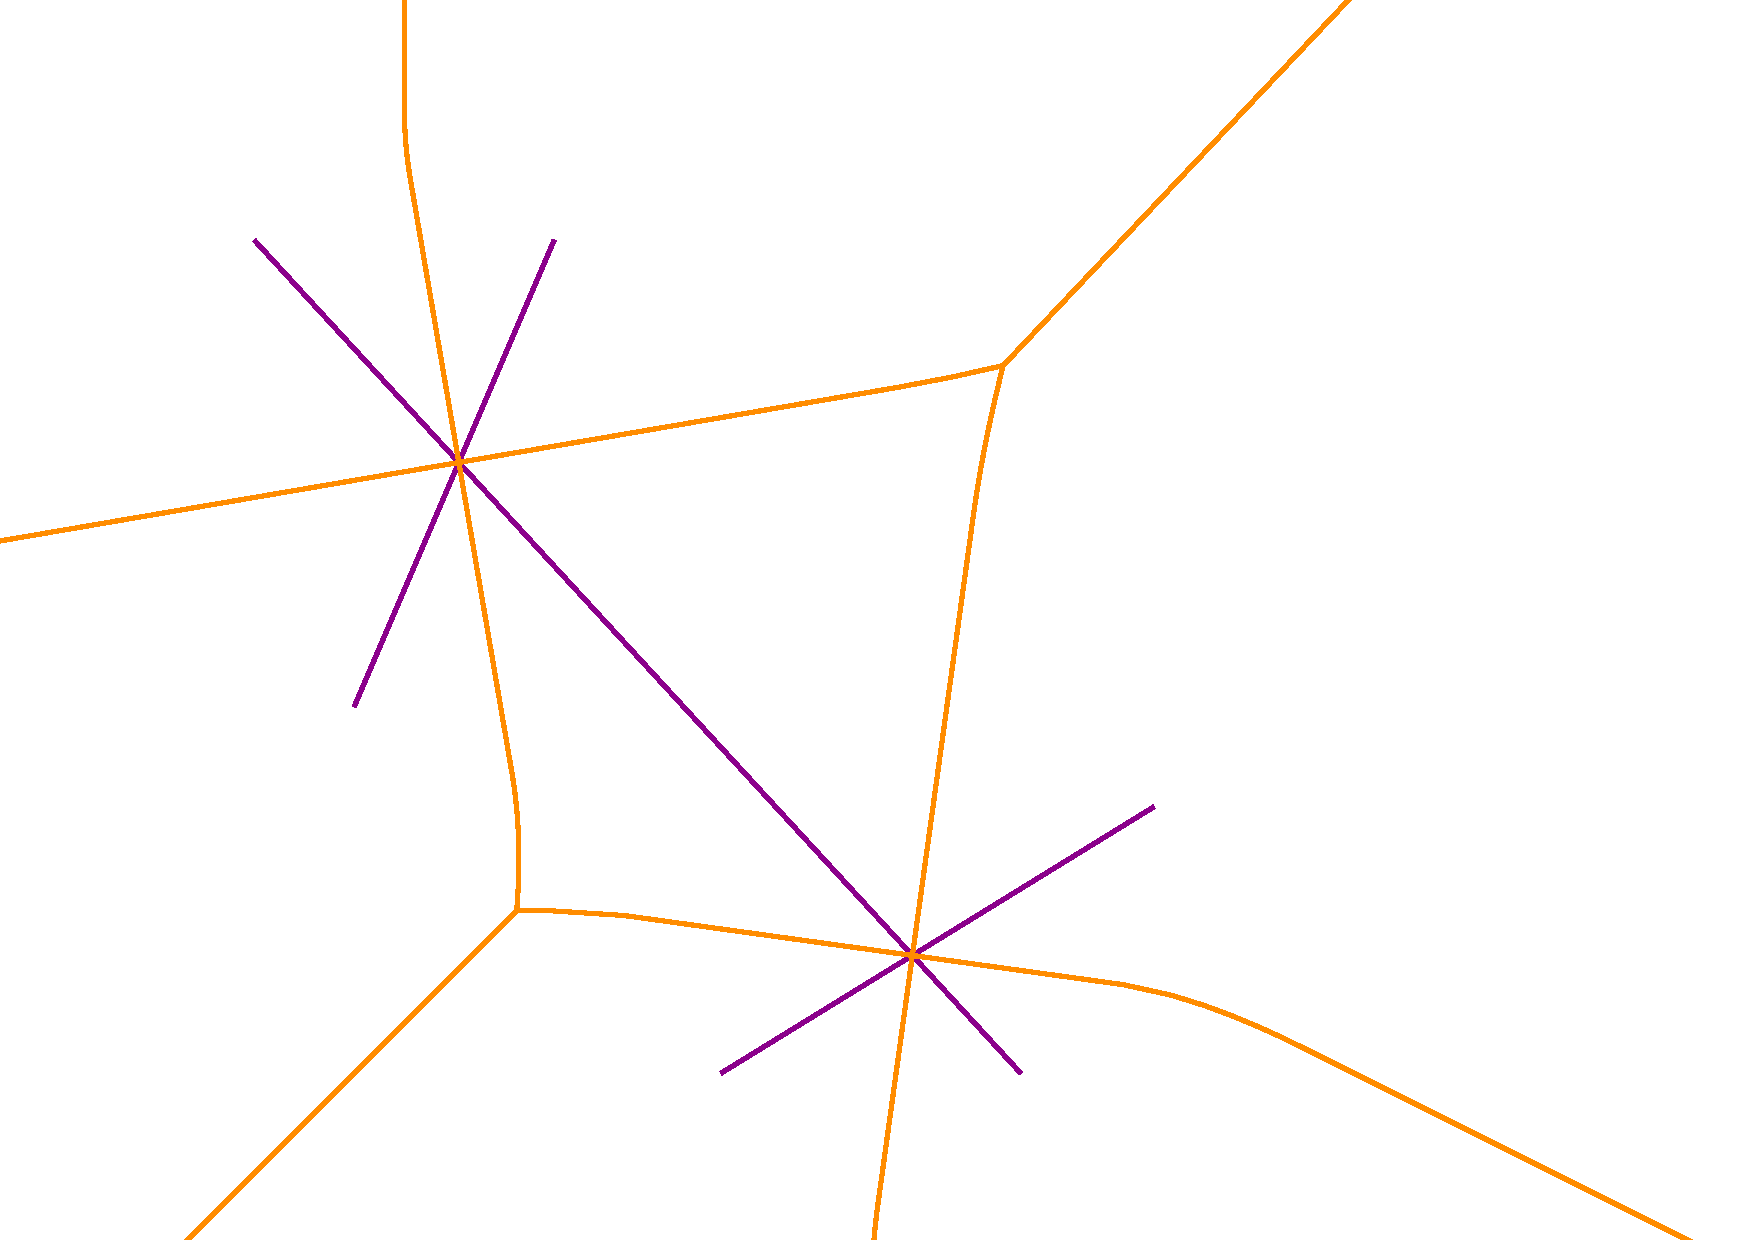
\includegraphics[width=\textwidth]{SVD_example}
        \caption{Nearest}
        \label{fig:SVD_example}
    \end{subfigure}
	\qquad
    \begin{subfigure}[b]{0.45\textwidth}
        
\includegraphics[width=\textwidth]{FSVD_example}
        \caption{Farthest}
        \label{fig:FSVD_example}
    \end{subfigure}
    \caption{Voronoi diagrams with line segments\label{fig:examples}}
	\end{figure}
	
	\subsection{CGAL and Ipelets}
	
	In this project two new functions were added to an Ipelet that already featured functions to construct Voronoi diagrams of points, Voronoi diagrams for segments, points and polygons using the \(L_{\infty}\) metric, farthest color and Hausdorff Voronoi diagrams.\par
	The two functions added are to construct, under \(L_{2}\) metric, the nearest or the farthest Voronoi diagram for line segments.\par
	For both cases the strategy used is to get the distance function of each segment as a surface, then take either the upper or the lower envelope of these surfaces (for FSVD and SVD respectively).
	
	\subsection{The envelopes strategy}
	For a single segment on the \(xy\)-plane, for every point plot on the \(z\) axis the distance of that point to the segment. This creates a 3D surface. For a point, this surface is simply a cone; for a segment, it's two haflcones originating at the endpoints of the segment and two planes originating from the inner part of the segment (figure \ref{fig:distance_function}).\par
	\begin{figure}[h]
    \centering
    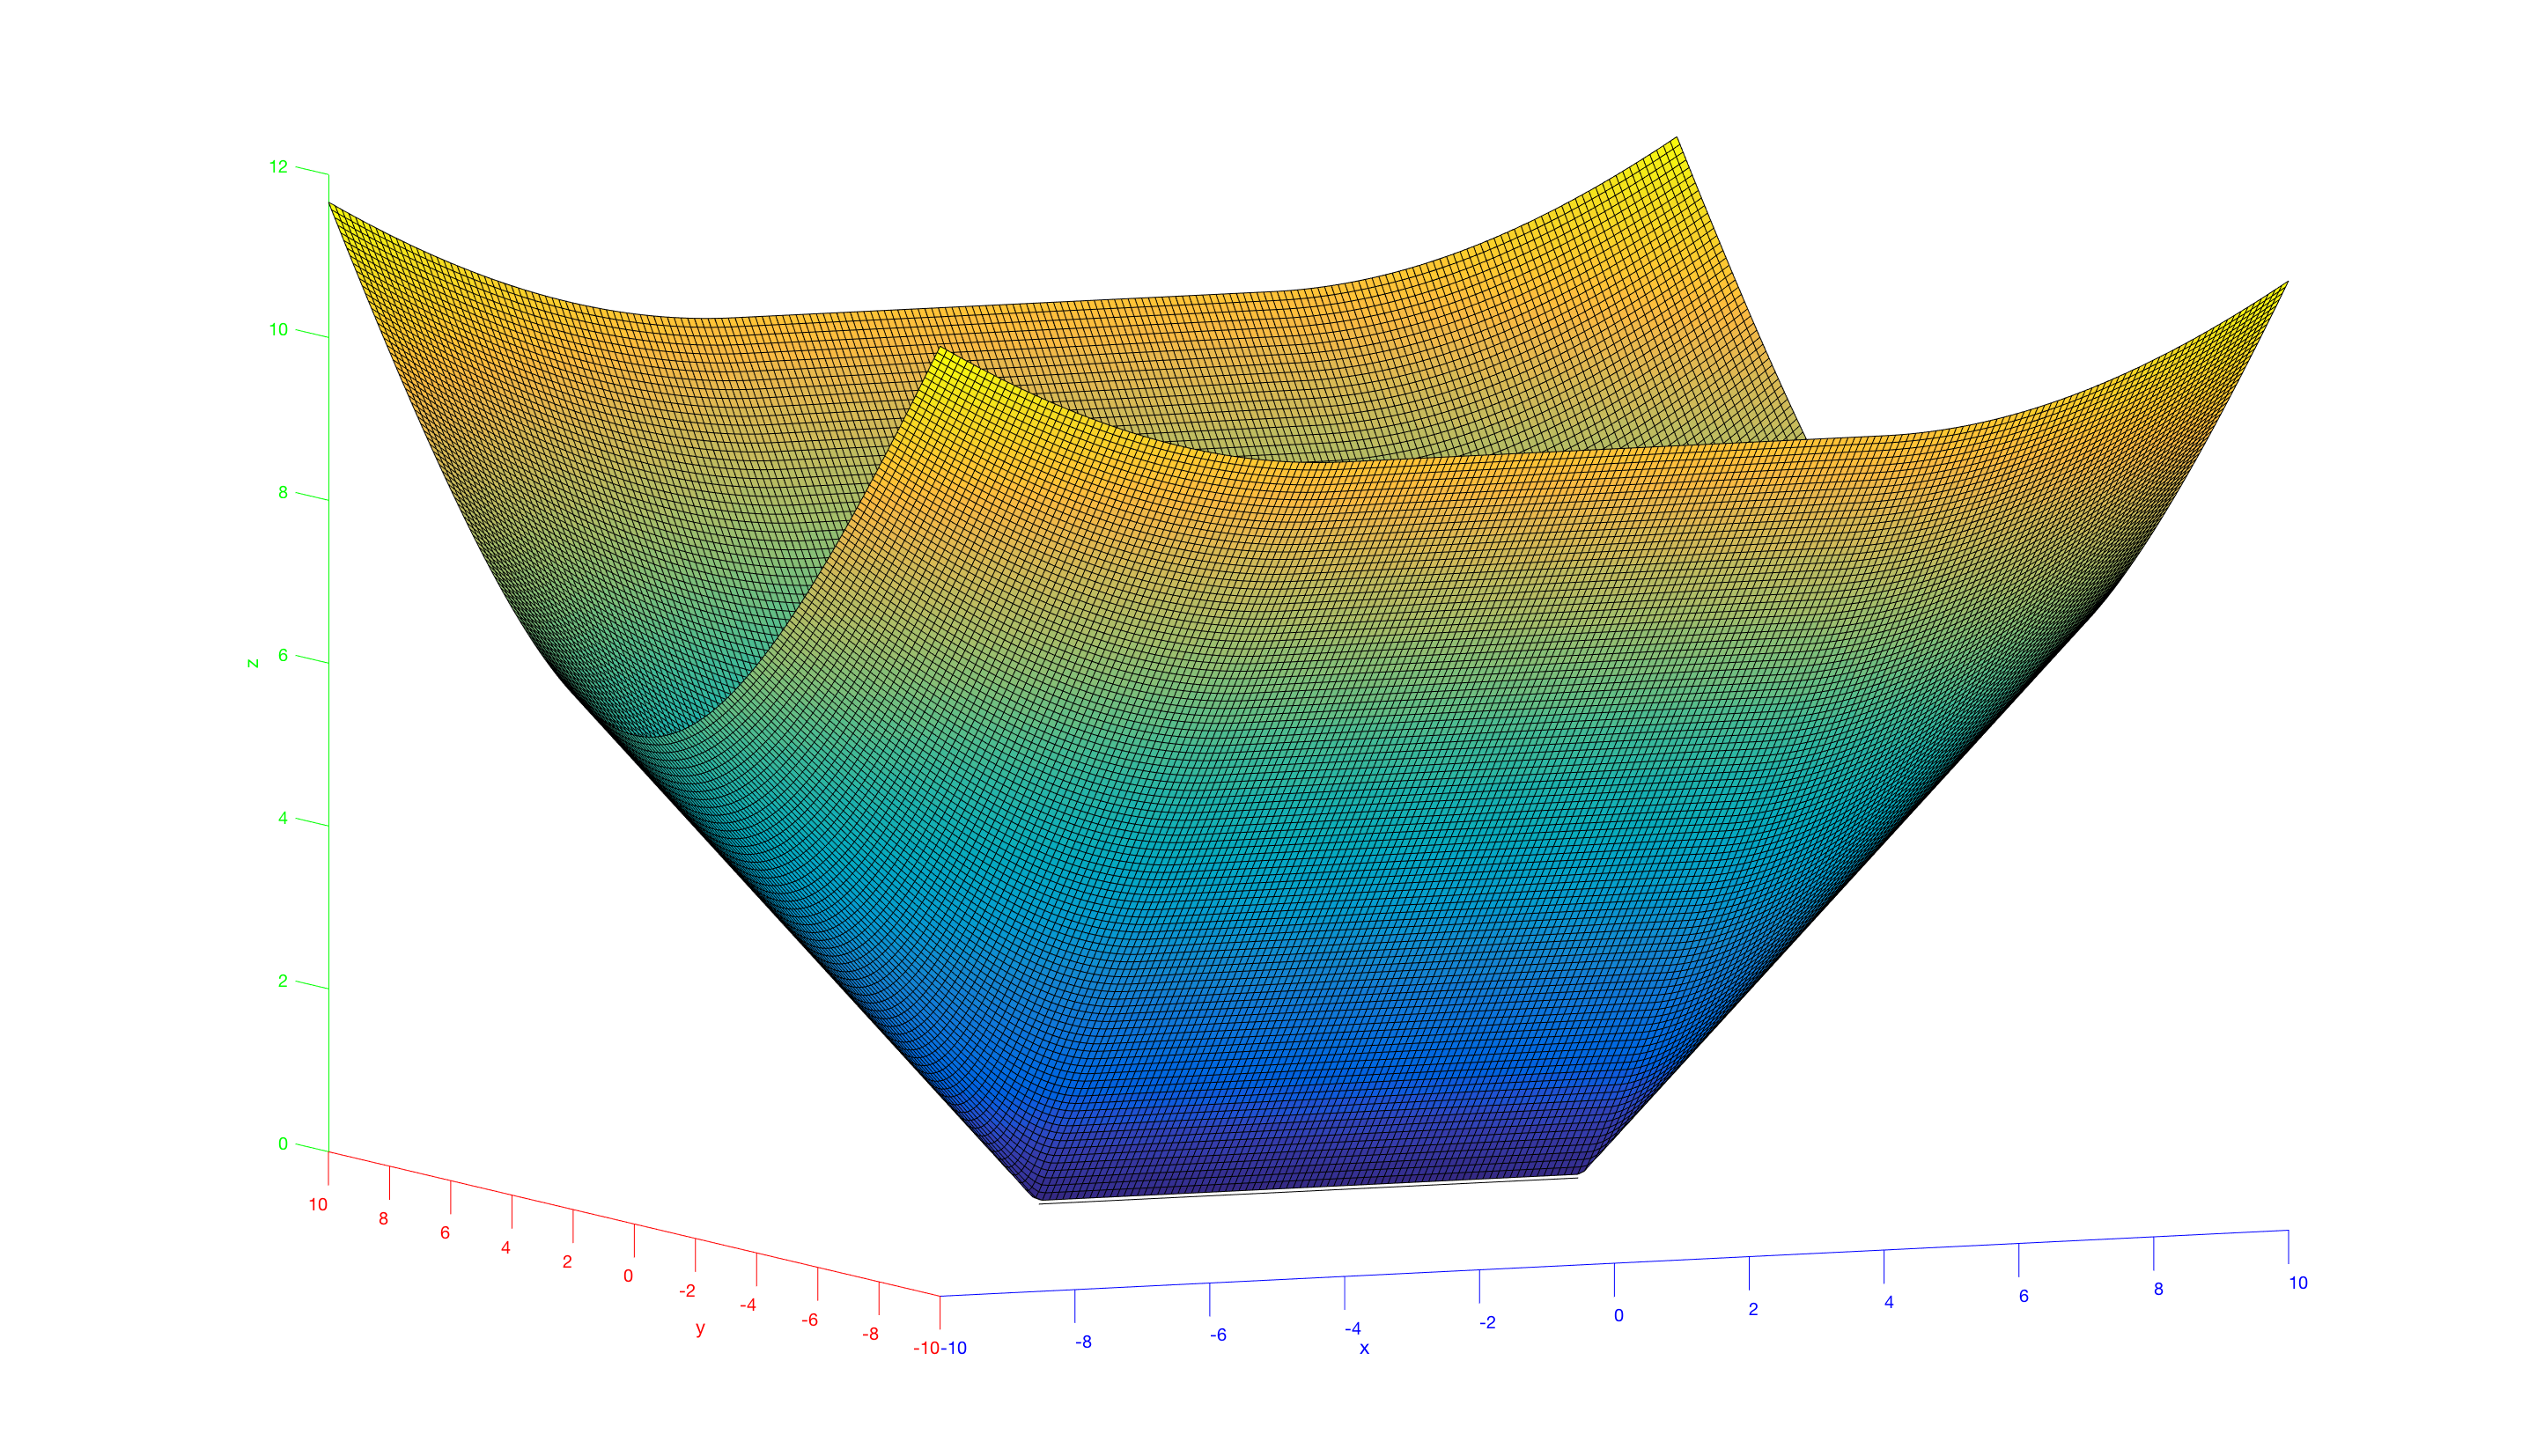
\includegraphics[width=0.8\textwidth]{distance_function}
    \caption{Distance function surface for a segment\protect\footnotemark \label{fig:distance_function}}
	\end{figure}
	\footnotetext{created using MATLAB script by Martin Suderland}
	For two distinct segments, these distance function surfaces intersect, and their intersection projected back onto the \(xy\)-plane is simply the planar euclidean bisector of the two segments.\par
	For many segments, given all their distance function surfaces, if the lower envelope is taken then the \(xy\)-projection of this envelope is the nearest Voronoi diagram, whereas the \(xy\)-projection of the upper envelope is the farthest Voronoi diagram.
	
	%____________________________________________________________

	\section{Envelope package and \cod{Envelope_diagram_2<EnvTraits>}}
	CGAL features a package to compute projections of envelopes. The methods \cod{upper_envelope_3} and \cod{lower_envelope_3} output their resulting \(xy\)-projection diagram in a \cod{Envelope_diagram_2} object.\par
	This diagram class is parametrised by a traits class that must define the geometry it handles; to do so, it needs to support computation of the projected boundary of a surface, the projection of the intersection of two surfaces, as well as other functions to determine the z-order of two surfaces in specific cases (more specifically, the traits class must be a model of the concept \cod{EnvelopeTraits_3}, specified on the \href{https://doc.cgal.org/4.9.1/Envelope_3/classEnvelopeTraits__3.html}{CGAL documentation}).\par
	There are already traits classes to support construction of envelopes of spheres, triangles and planes, but these did not include what we needed for FSVD, so a new class needed to be developed.
	
	\subsection{Traits class \cod{L2_segment_voronoi_traits_2<ArrTraits_2>}}
	The \cod{EnvelopeTraits_3} concept allows the surfaces to be any kind of object, as long as the required functions do their task. Because of this, for FSVD (and SVD too, they can use the same traits class) the surfaces are simply the segments themselves, since they contain all the information needed for the computations.\par
	In the function that requires to compute the projected intersection of two surfaces, we can in fact simply compute the planar euclidean bisector of the two segments.\par
	The bisector is formed, in the general case, by unbounded rays, segments and parabolic arcs (figure \ref{fig:areas_of_influence}).\ppar
	\begin{figure}[h]
    \centering
    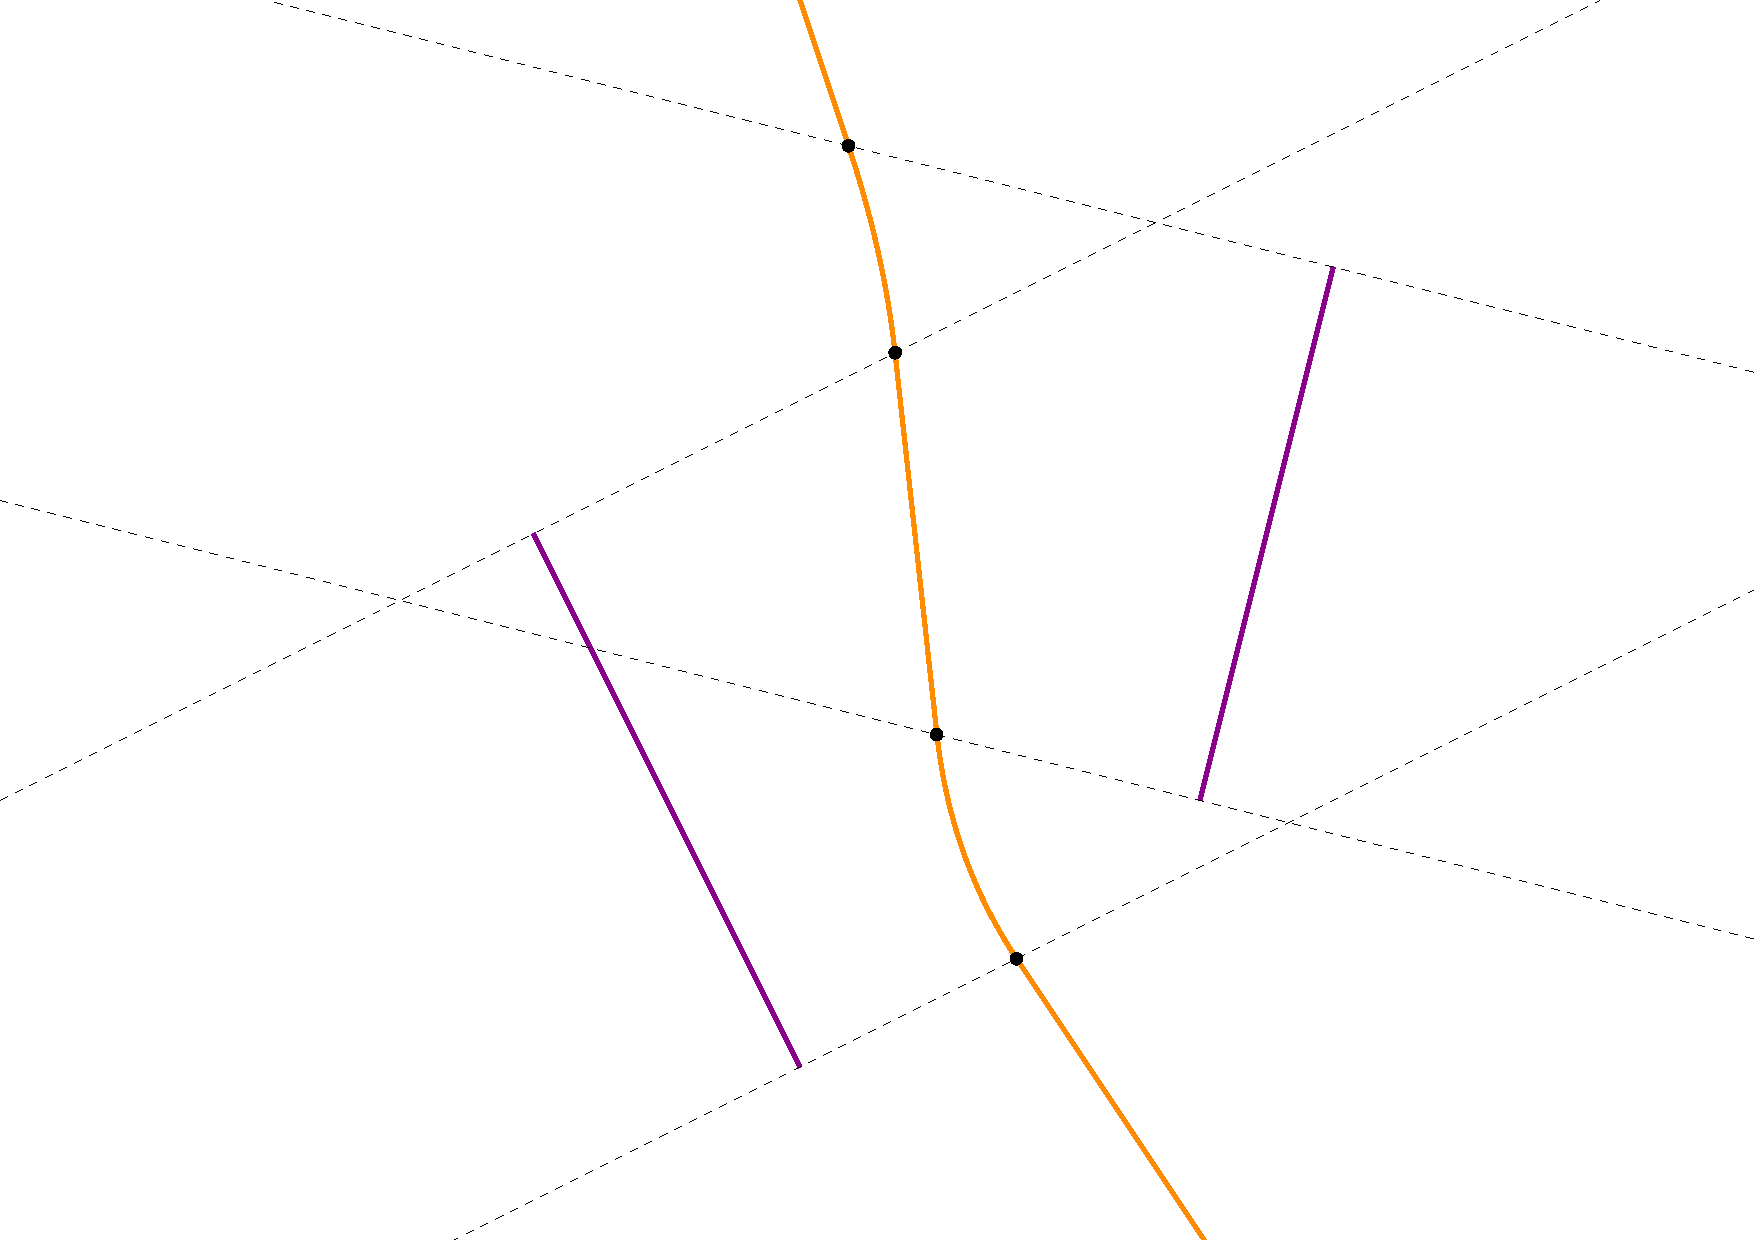
\includegraphics[width=0.8\textwidth]{areas_of_influence}
    \caption{Different parts of the bisector\label{fig:areas_of_influence}}
	\end{figure}
	Notice how the parts of the bisector are delimited by the lines orthogonal to the segments at their endpoints. For a single segment, these two lines divide the plane in three parts: the points closest to the source of the segment, the points closest to the inner part of the segment, the points closest to the target.\ppar
	The model of the concept \cod{EnvelopeTraits_3} that was developed is  \cod{L2_segment_voronoi_traits_2} and is parametrised by an Arrangements class from which it inherits, similarly to how the already available model \cod{Env_sphere_traits_3} for envelopes of spheres does; again similarly, the Arrangements class used is \cod{Arr_conic_traits2}.\par
	This Arrangements class defines the geometry of the edges of the diagram, as well as methods for computation of intersections and predicates.
	
	\subsection{Arrangement traits class \cod{Arr_conic_traits2}}
	This class was chosen because it supports construction and computation using conic curves, needed because of the parabolic arcs in the planar euclidean bisector of two segments; such arcs are present in the part of the bisector that is closest to one of the segments' inner part and to one the other segment's endpoints (see figure \ref{fig:areas_of_influence}).\par
	The curves need to be closed conic arcs lying on a supporting conic curve defined by the equation:
	\[
		rx^{2} + sy^{2} + txy + ux + vy + w = 0 
	\]
	According to the specification (available on the \href{https://doc.cgal.org/latest/Arrangement_on_surface_2/classCGAL_1_1Arr__conic__traits__2.html}{CGAL documentation}), the coefficients (\(r, s, t, u ,v, w\)) need to be all rational numbers. This is because by enforcing this, all intersections between such conic arcs are guaranteed to be algebraic numbers of degree at most 4, and the traits class is optimised for operations with these numbers.\par
	If the supporting conic is not a closed curve such as a circle or an ellipse, and it our case it never is (because it's either a parabola or a line for the straight parts of the bisector), then two endpoints have to be provided. This poses a problem with the unbounded rays (the first and last parts of the bisector, again see figure \ref{fig:areas_of_influence}), because they only have one endpoint.\par
	To obviate this, the rays were cut off at an arbitrary distance: imagine this as if the distance surfaces were not unbounded, but were all limited inside the same huge square. Because of this, the traits class \cod{L2_segment_voronoi_traits_2} also constructs a projected boundary for all surfaces (the same for all of them).
	

	\subsection{\cod{Parabola} class}
	A \cod{Parabola} class was implemented to support construction of parabolas, computation of intersection with lines and construction of arcs on the parabolas. Other predicates such as \cod{has_on} were also implemented.\par
	The only constructor for a \cod{Parabola} object takes a focus point and a directrix line. These are defined as the endpoint of one segment and the supporting line of the other segment accordingly (see figure \ref{fig:parabola}, parabola in green).
	\begin{figure}[h]
    \centering
    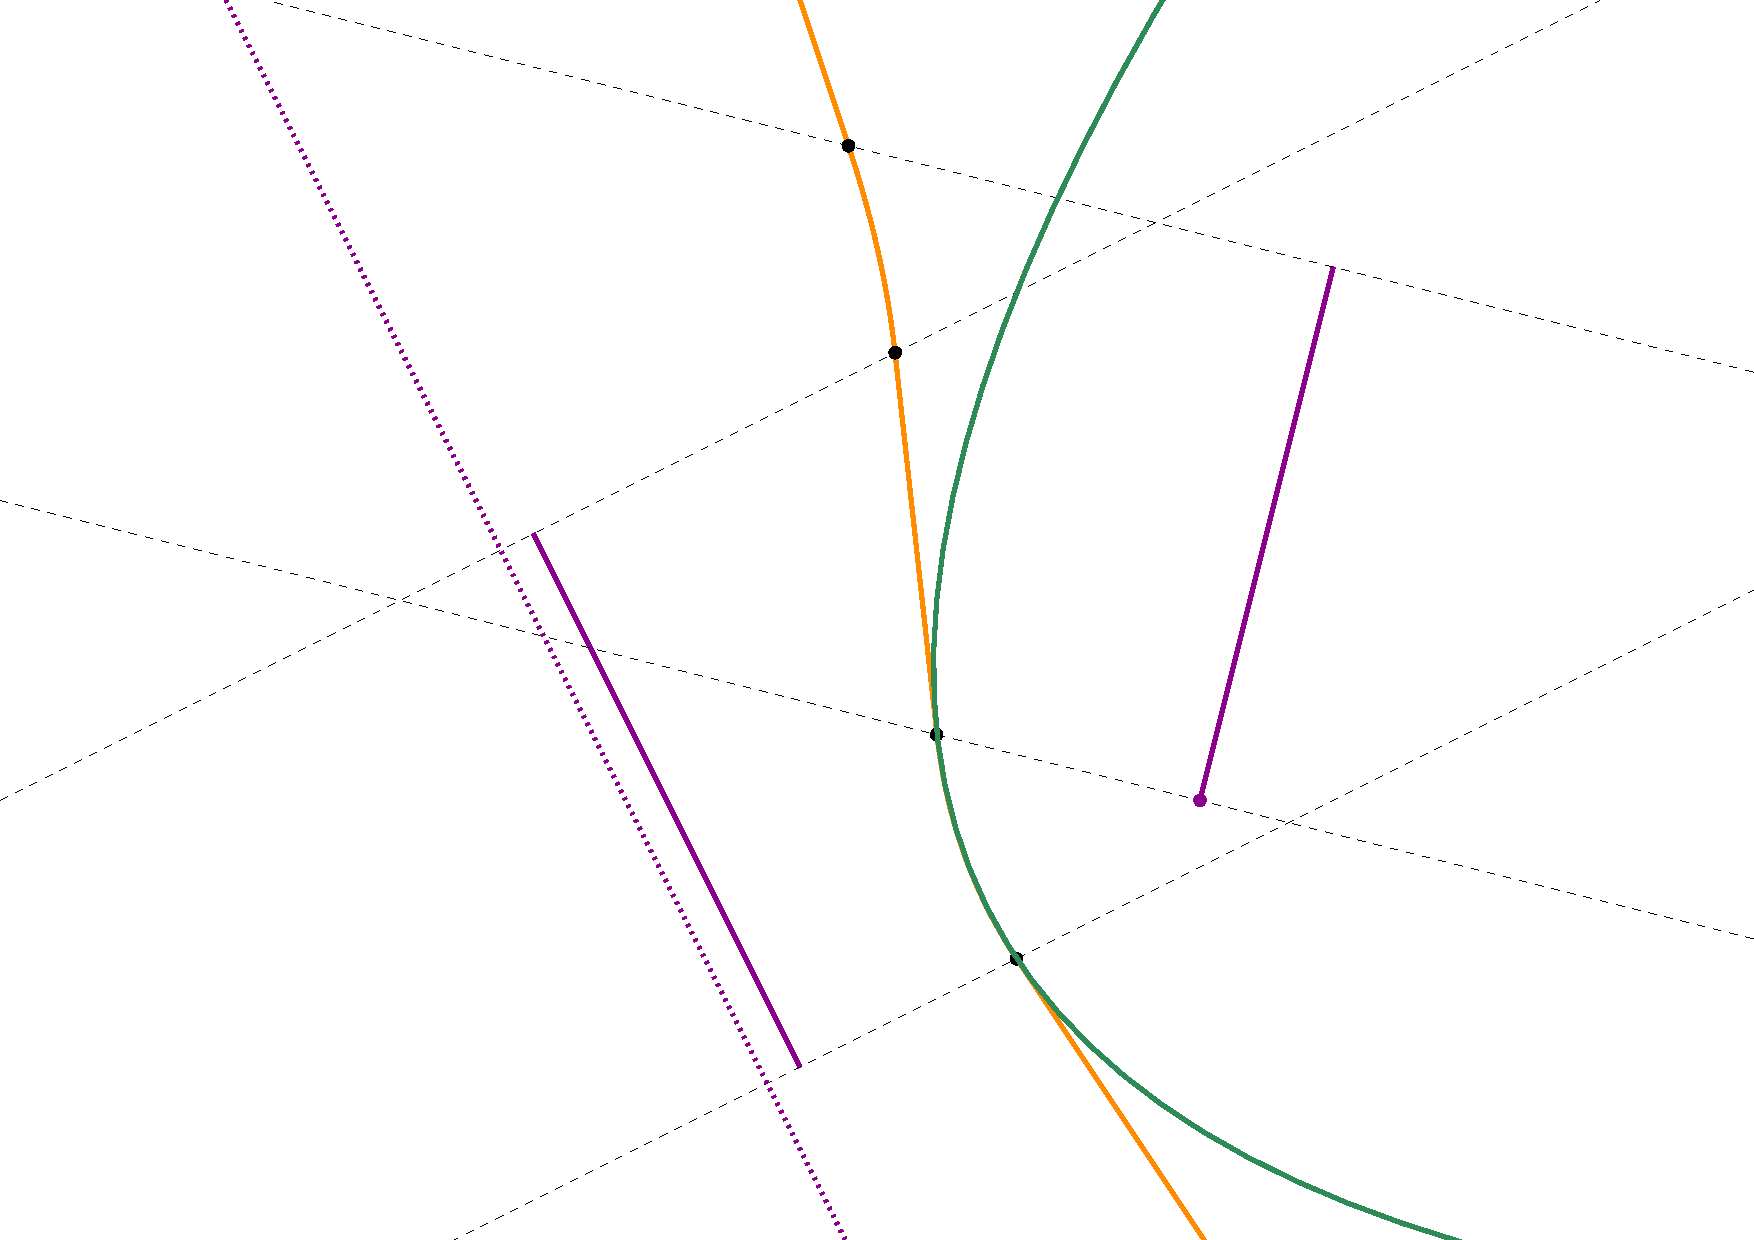
\includegraphics[width=0.8\textwidth]{parabola}
    \caption{A parabola defined by a supporting line (dotted) and the highlighted endpoint \label{fig:parabola}}
	\end{figure}
	
	
	%____________________________________________________________

	\section{Bisector computation}
	
	\subsection{Unbounded rays}
	
	\subsection{Internal part}
	
	\subsection{Challenges and solutions}
	
	%____________________________________________________________
	
	\section{Results and future work}
	
	\subsection{Ipelet issues}
	
	\subsection{Known limitations}
	
	\subsection{Alternatives}
	
	\subsubsection{\cod{Arr_linear_segment_traits_2}}
	
	\subsubsection{Own Arrangements class}
	
\end{document}
